\documentclass{article}%
\usepackage[T1]{fontenc}%
\usepackage[utf8]{inputenc}%
\usepackage{lmodern}%
\usepackage{textcomp}%
\usepackage{lastpage}%
\usepackage[head=40pt,margin=0.5in,bottom=0.6in]{geometry}%
\usepackage{graphicx}%
%
\title{\textbf{Cinco reporteros fueron retenidos por el Dgcim}}%
\author{El Nacional Web}%
\date{24/09/2018}%
%
\begin{document}%
\normalsize%
\maketitle%
\textbf{URL: }%
http://www.el{-}nacional.com/noticias/sociedad/cinco{-}reporteros{-}fueron{-}retenidos{-}por{-}dgcim\_253035\newline%
%
\textbf{Periodico: }%
EN, %
ID: %
253035, %
Seccion: %
Sociedad\newline%
%
\textbf{Palabras Claves: }%
Sociedad\newline%
%
\textbf{Derecho: }%
1.2, %
Otros Derechos: %
, %
Sub Derechos: %
1.2.1.3\newline%
%
\textbf{EP: }%
SI\newline%
\newline%
%
\textbf{\textit{Los ciudadanos se encontraban en la zona investigando sobre la detención de Isnardo Bravo}}%
\newline%
\newline%
%
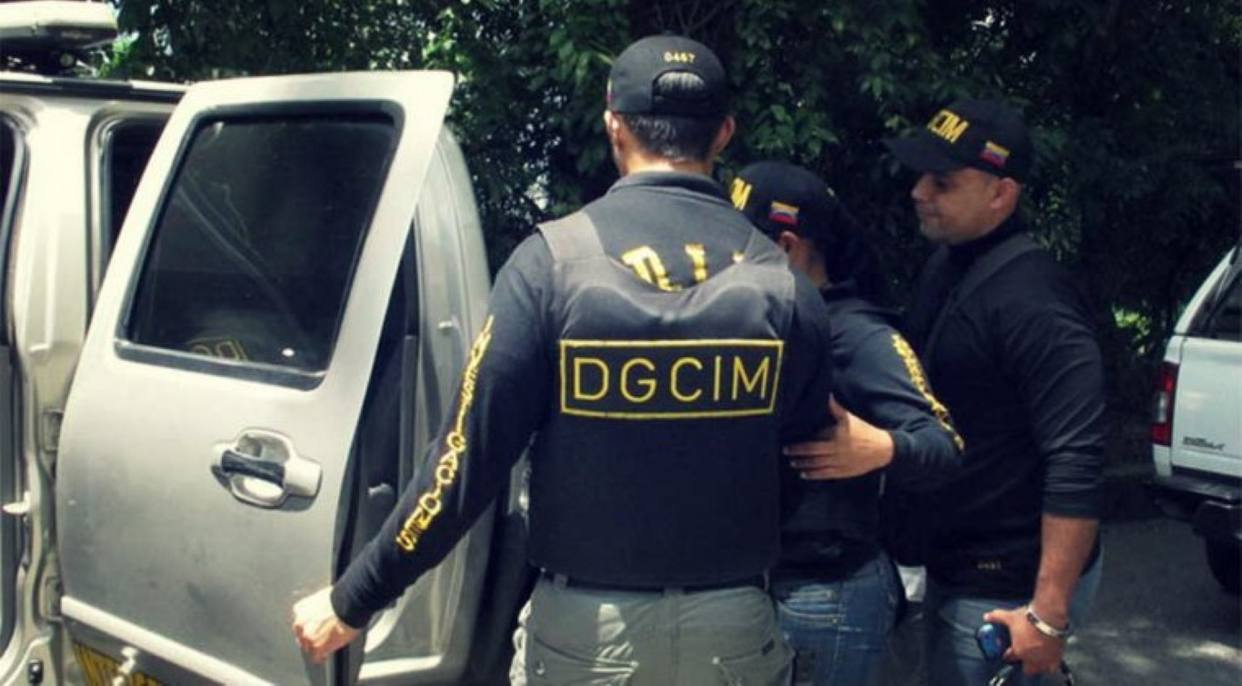
\includegraphics[width=300px]{151.jpg}%
\newline%
%
Varios reporteros venezolanos fueron detenidos este lunes en los alrededores de la Dirección General de Contrainteligencia Militar (Dgcim) en Boleita, mientras buscaban información sobre Isnardo Bravo, periodista de~VPI.%
\newline%
%
“Nuestra reportera Ana María Rodríguez Brazón y su camarógrafo Edgar Hernandez fueron abordados por funcionarios del DGCIM mientras se encontraban a unos metros de su sede, esto con el fin de informar sobre el caso de nuestro colega Isnardo Bravo”, indicó~VPI~en suTwitter.%
\newline%
%
Por su parte, el Sindicato Nacional de Trabajadores de la Prensa de Venezuela (SNTP) agregó a Luis Gonzalo de~NTN24; Luis Laya, de~Venepress~e Irene Mejía de~Caraota Digital~a la lista de los profesionales que fueron detenidos por las autoridades.%
\newline%
%
A Bravo se le revocó el pasaporte en el Aeropuerto Internacional Simón Bolívar en Maiquetía, estado Vargas, este lunes cuando se disponía a viajar junto a su familia afuera del país.%
\newline%
%
Funcionarios de la Dgcim trasladaron al periodista desde el aeropuerto hasta la sede el organismo en Boleíta, municipio Sucre en el estado Miranda.%
\newline%
%
\end{document}